\newcommand{\light}[1]{\textcolor{gray}{#1}}

\frame{
    \frametitle{Contents}
    \begin{enumerate}
    \item About Me
        \vspace{0.5cm}
    \item Introduction
        \vspace{0.5cm}
    \item Measurement
        \vspace{0.5cm}
    \item Simulation
        \vspace{0.5cm}
    \item Summary
        \vspace{0.5cm}
    \end{enumerate}
}

\frame{
   \frametitle{About Me}
   \begin{columns}
   \column{0.5\textwidth}
   \centering
   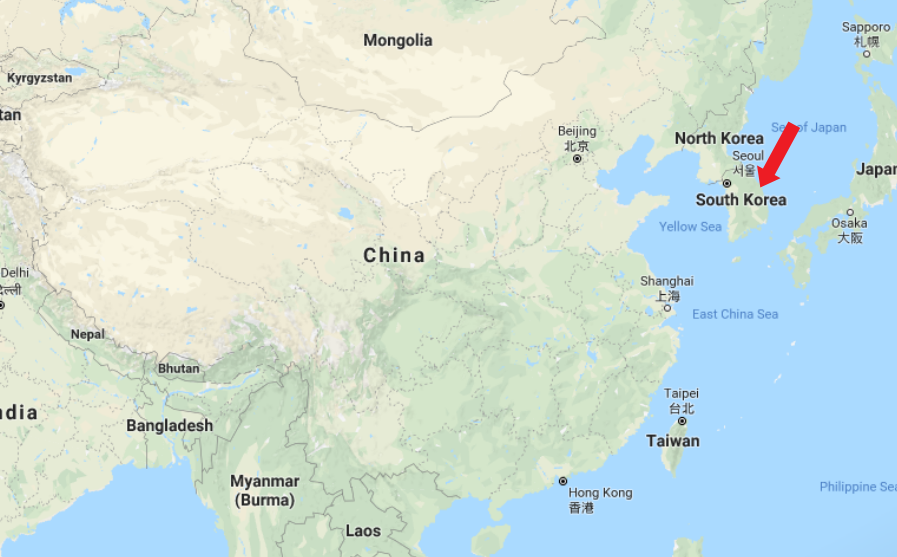
\includegraphics[width=2.3in]{pictures/mymap.png}
   \column{0.5\textwidth}
   \begin{itemize}
    \item From South Korea
      \vspace{0.3cm}
    \item Kyungpook National University, Daegu 
      \vspace{0.3cm}
    \item First year master course student in experimental high energy physics
   \end{itemize}
   \end{columns}
}

%\frame{
%   \frametitle{Overview}
%   \begin{itemize}
%    \item Proposal to instrument the UX85A cavern with a set of tracking layers: \href{https://arxiv.org/pdf/1708.09395}{\textcolor{blue}{CODEX-b}}.
%      \vspace{0.2cm}
%.   \item Enhances LHCb's LLP (long-lived particles) search capabilities. Installation timeline $\sim $LS3.
%      \vspace{0.2cm}
%    \item Several other proposals for HL-LHC aligned w/ ATLAS/CMS: MATHUSLA, FASER, MILLIQAN...
%      \vspace{0.2cm}
%    \item CODEX-b simulation for reach studies need actual measurements of the background inside the cavern. Suitable project for a summer student (Jongho Lee).
%   \end{itemize}
%}


\frame{
    \frametitle{Equipment setup...}
        \begin{columns}
        \column{0.7\textwidth}
          \begin{itemize}
                \item Two $30\times30\times2$~cm wrapped plastic scintillators + PMT + mechanical stand (thanks to Raphael).
          \end{itemize}
      \vspace{0.1cm}
      \centering
      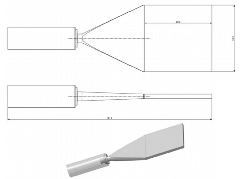
\includegraphics[width=2.3in]{figs/intro/scintillators}
          \begin{itemize}
                \item PMT's: HV crate and read out by scope. Setup tested w/ cosmics in VeloLab before transporting to pit (thanks to Heinrich). 
          \end{itemize}
        \column{0.3\textwidth}
            \centering
        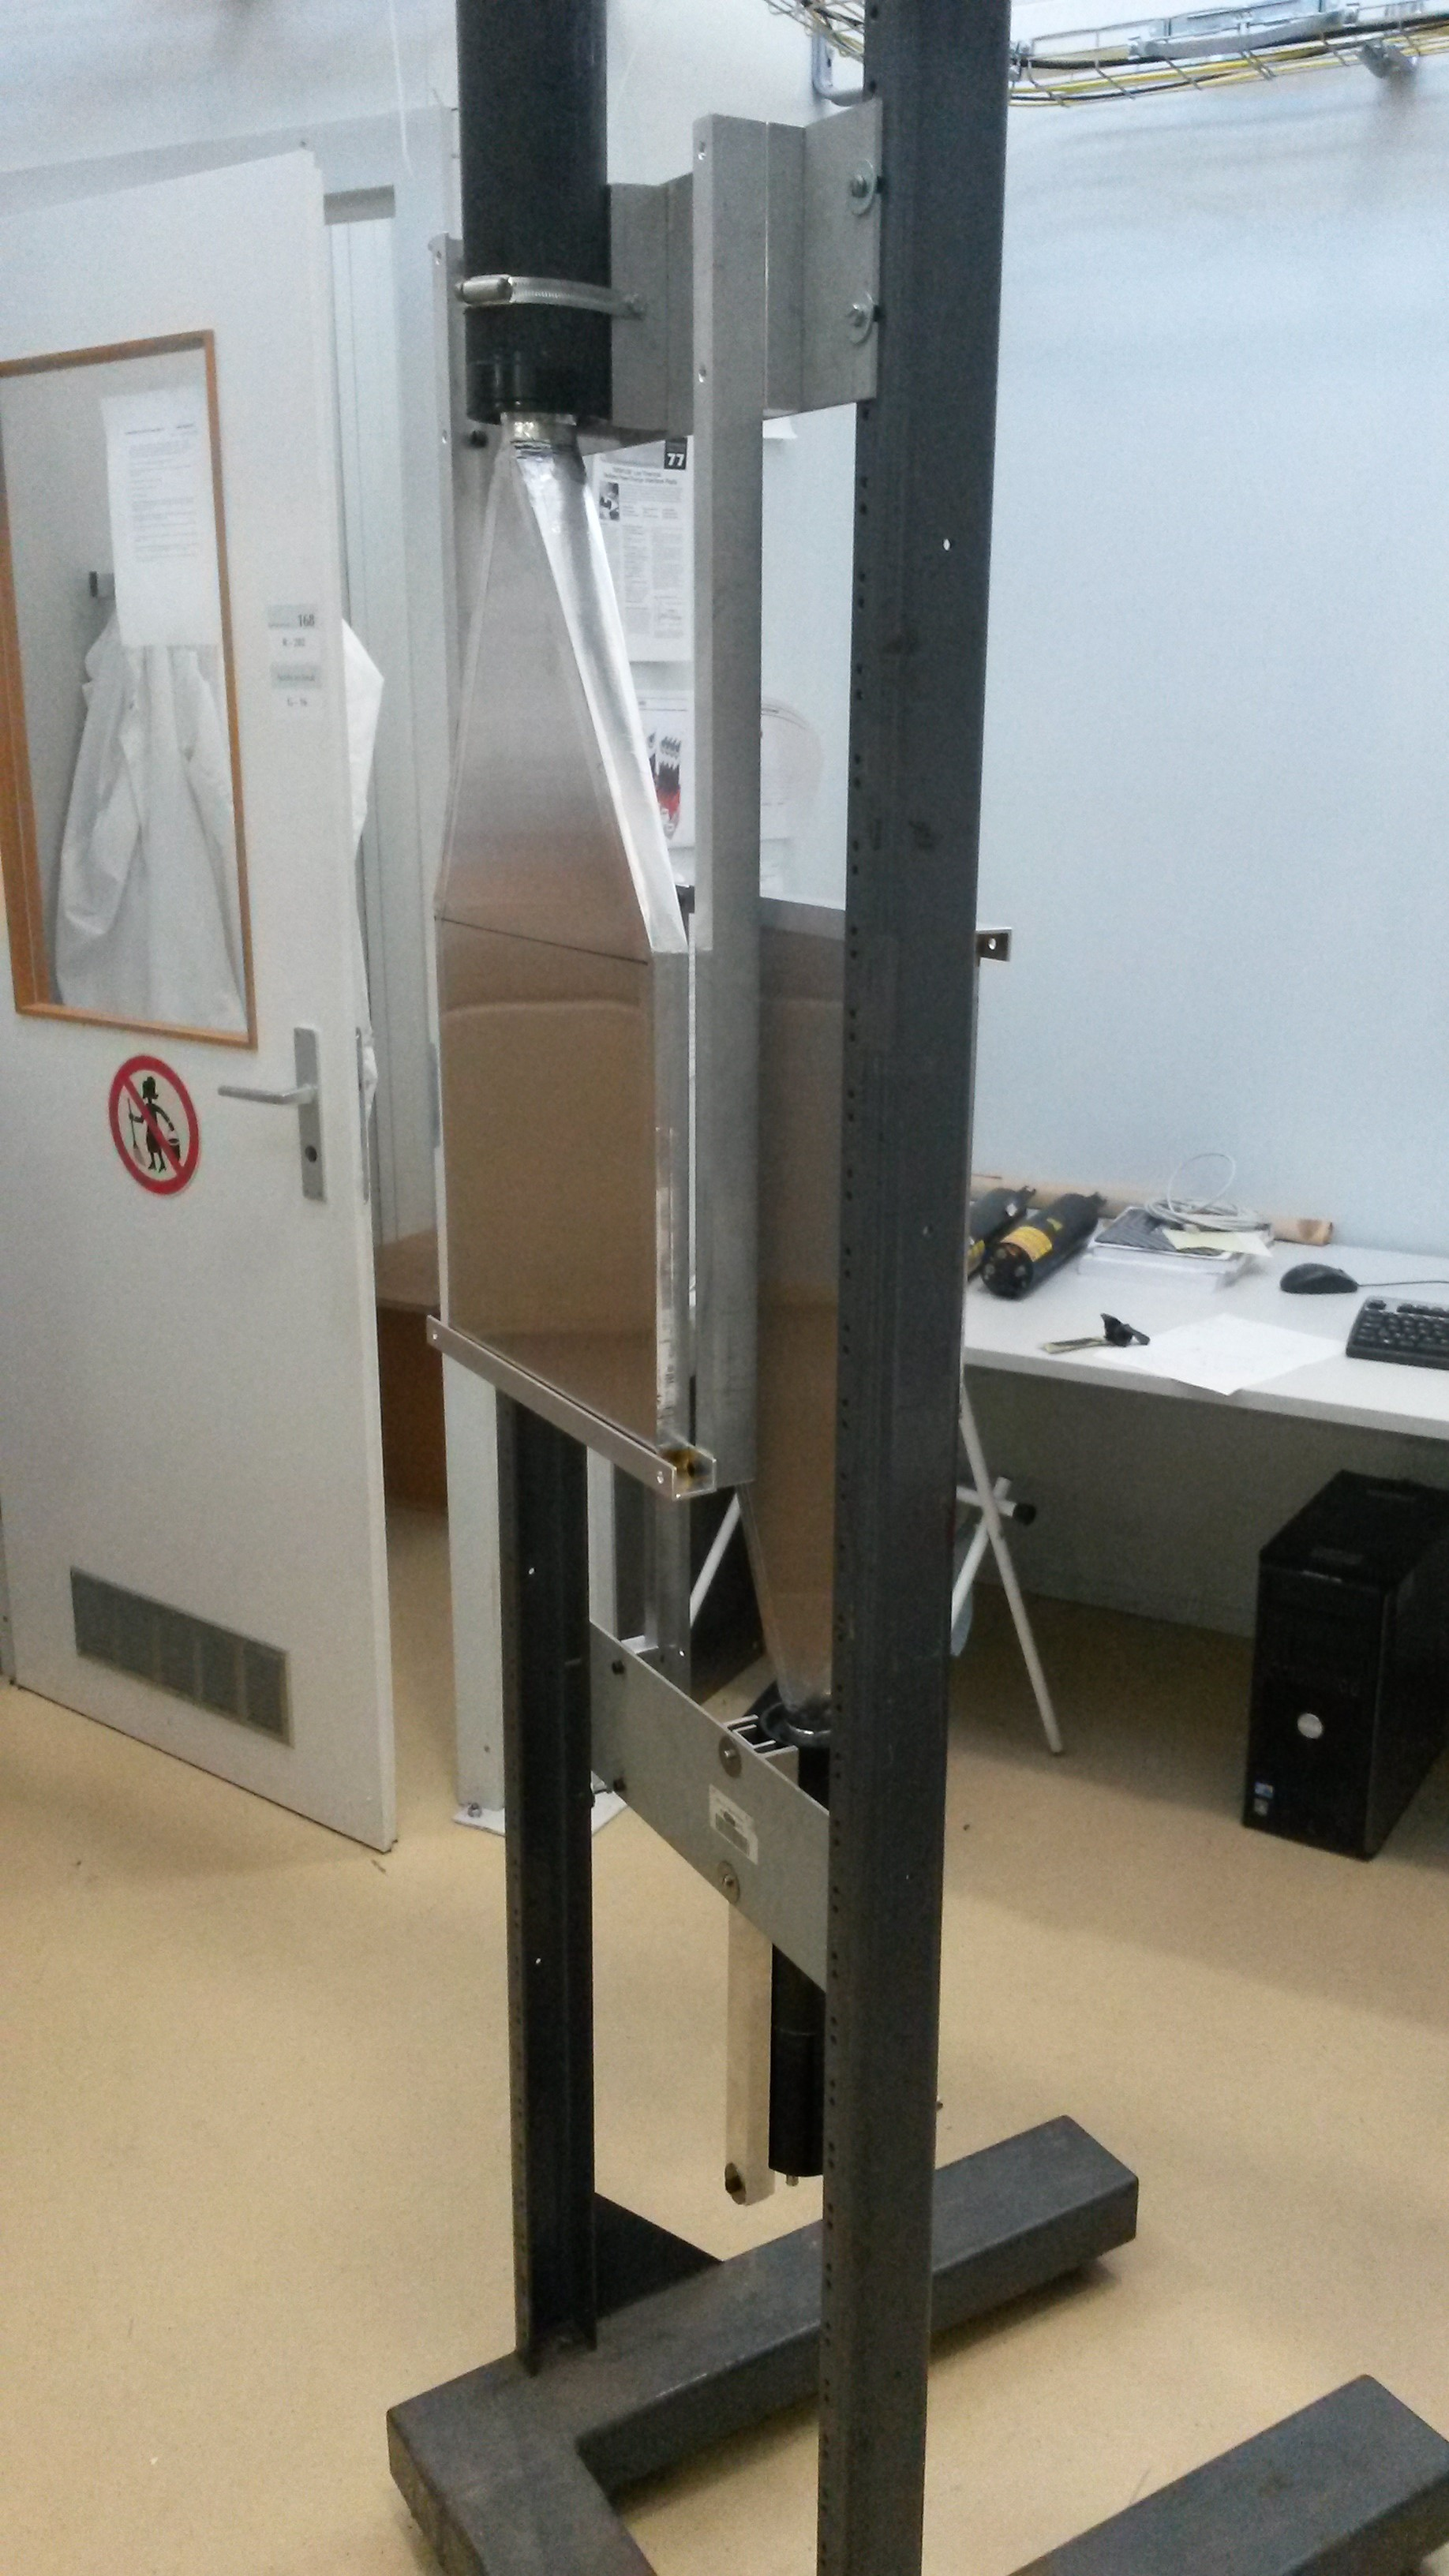
\includegraphics[width=0.8in]{figs/intro/mechanical_stand}\\
        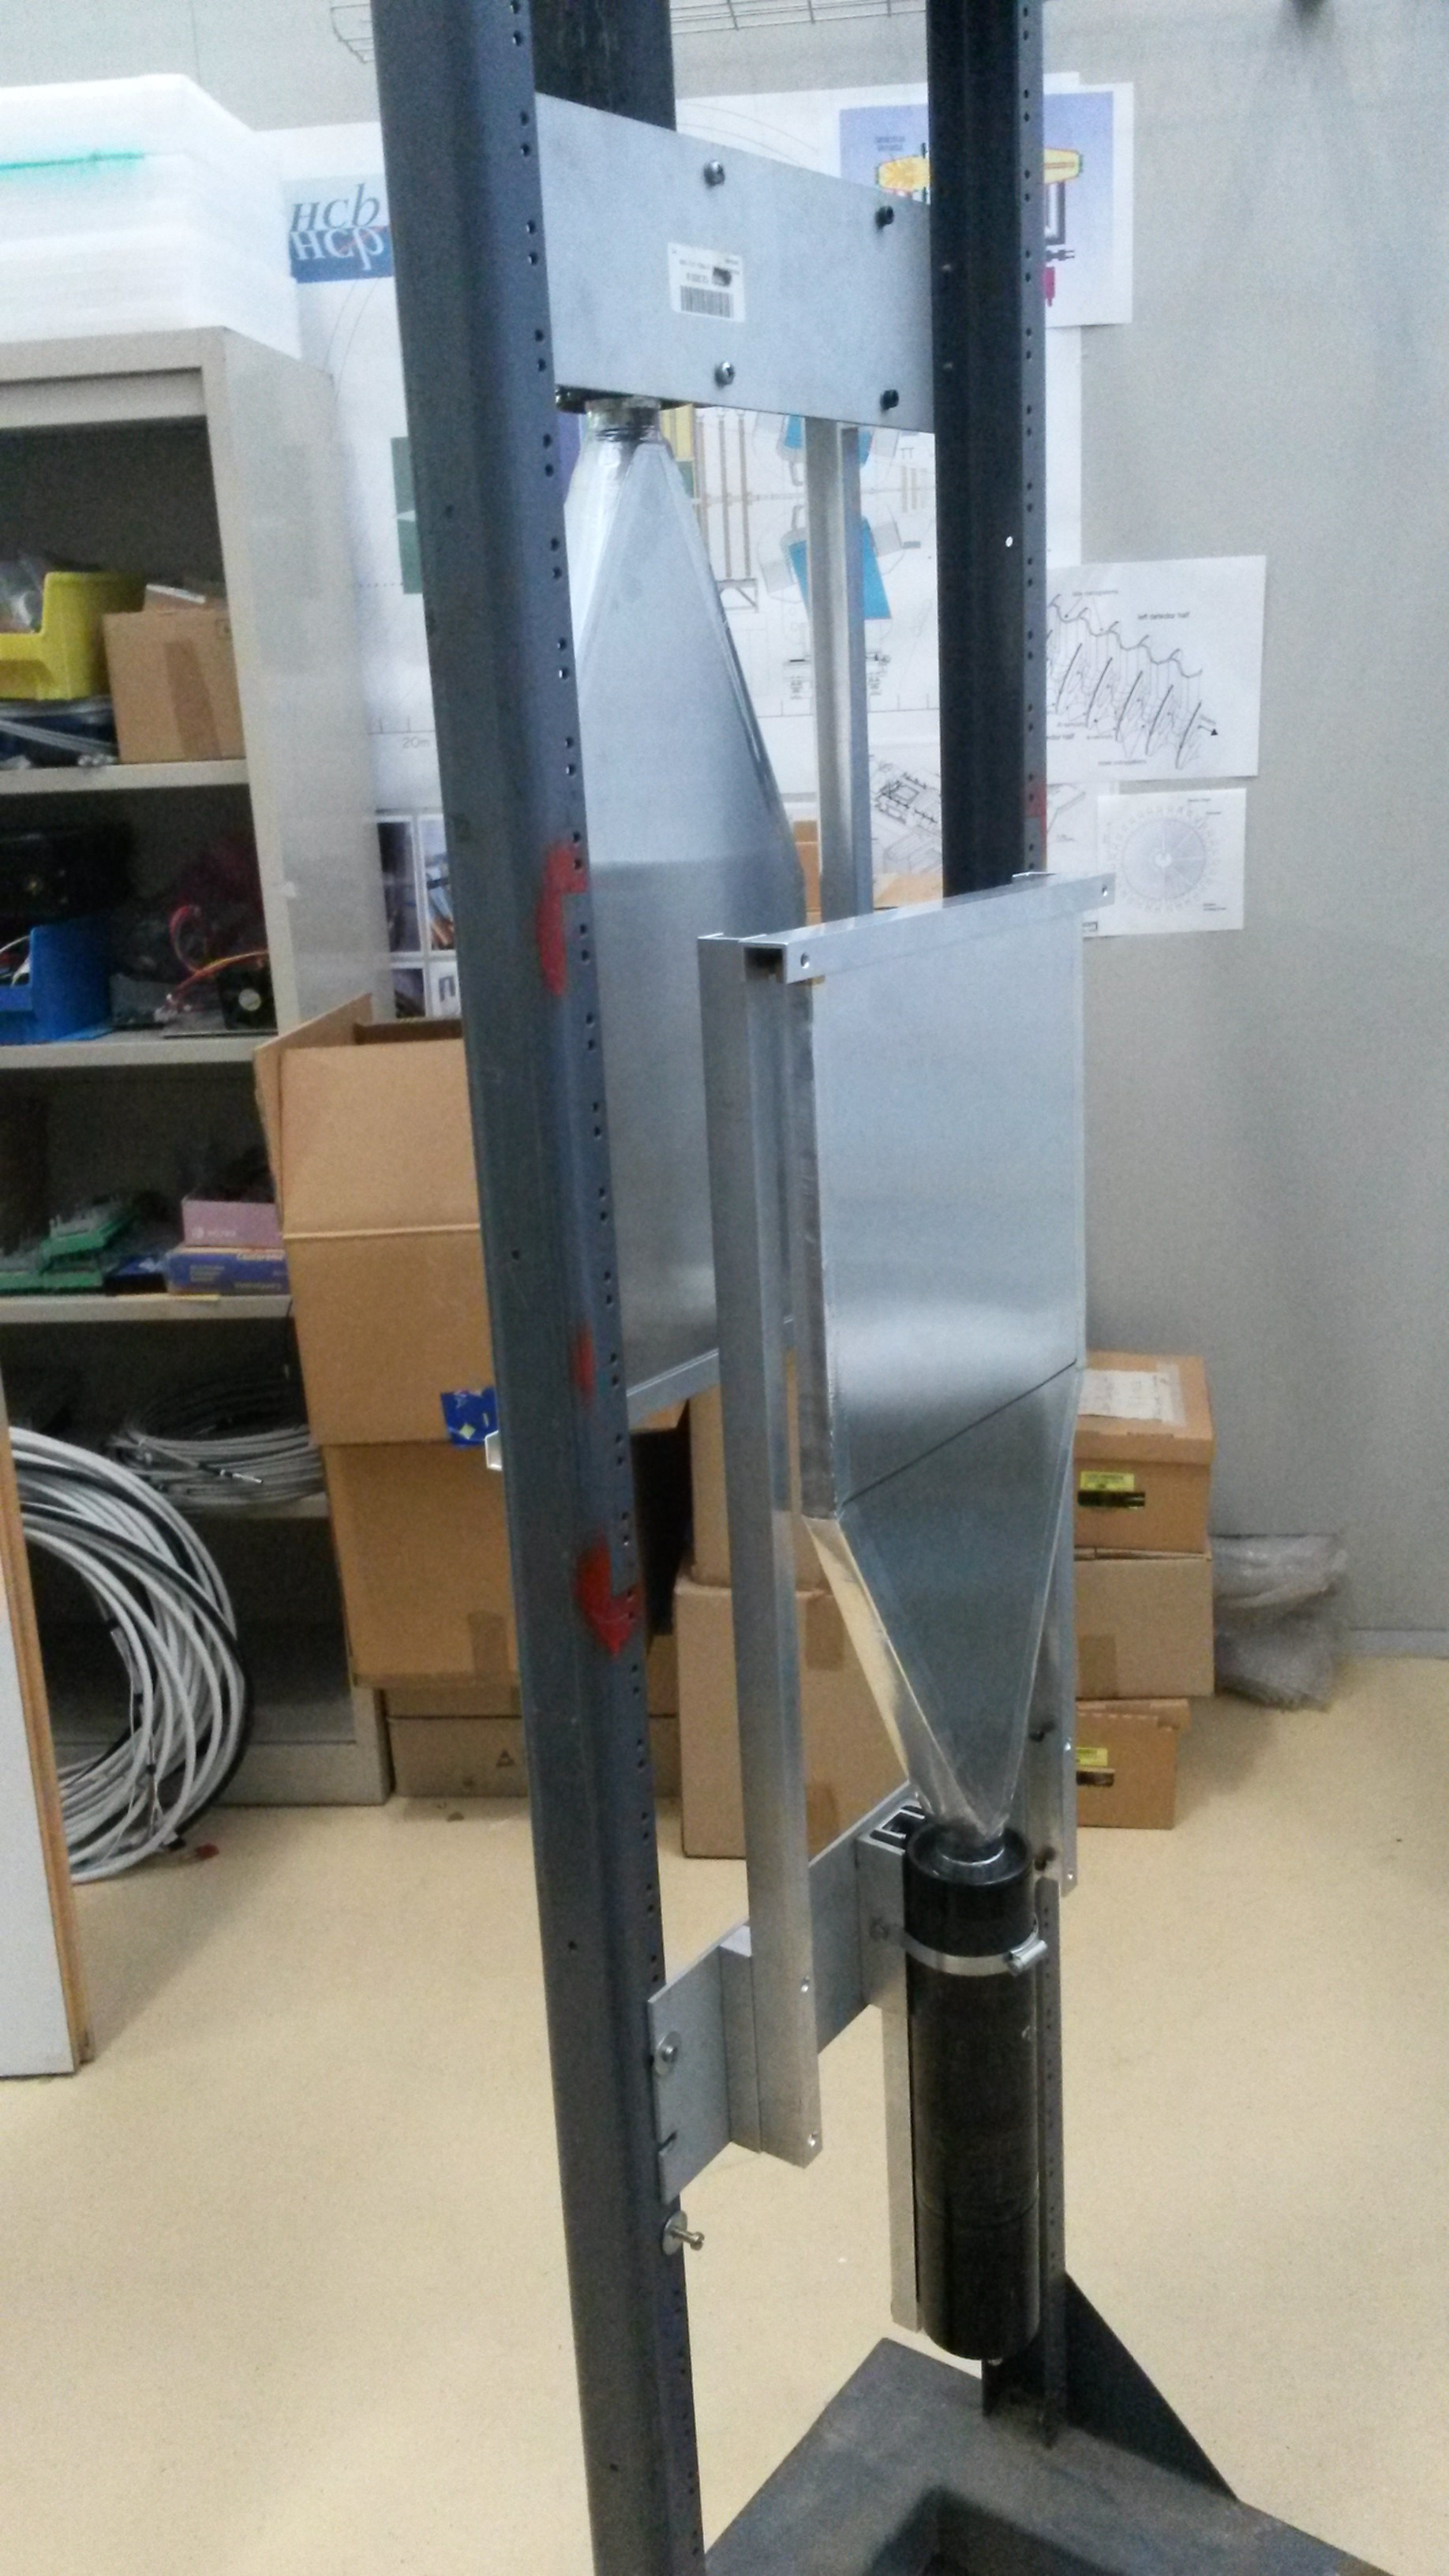
\includegraphics[width=0.8in]{figs/intro/mechanical_stand_1}
    \end{columns}
}



\frame{
    \frametitle{Measurements around D3}
     \begin{itemize}
       \item D3 platform is suitable...around the beam level and behind the shield wall. 
       \vspace{0.3cm}
       \item Measure counts at various positions and orientations. Calibrate simulation. 
       \vspace{0.3cm}
       \item Started actual measurements on 25th July during MD. Should be done by today.
       \vspace{0.3cm}
       \item Quite smooth data taking overall.
     \end{itemize}
}

\frame{
   \frametitle{Setup around D3}
    \begin{columns}
        \column{0.5\textwidth}
            \centering
        \includegraphics[angle=-90,width=5cm]{figs/codexb/D3_front_central2.jpg}
        \column{0.5\textwidth}
            \centering
        \includegraphics[angle=-90,width=5cm]{figs/codexb/D3_back_otherCorner1.jpg}
    \end{columns}
}

\frame{
   \frametitle{Sample DQ and analysis}
     \begin{itemize}
       \item Analysis and simulation ongoing. Sanity checks look good. 
       \item Hit rate across during and after \textcolor{red}{fill 7017} ends (Fri 3rd Aug).
     \end{itemize}
      \centering
      %\includegraphics[width=8cm]{/afs/cern.ch/user/b/bdey/lxwork/private/CODEX-b/CodexB/scripts/Friday_D3_center_pos.png}
}


\frame{
   \frametitle{Summary}
     \begin{itemize}
       \item Quite different experience from testbeam campaign. 
       \vspace{0.3cm}
       \item Unique dataset IMO...can be used by other LLP proposals.  
       \vspace{0.3cm}
       \item Analysis ongoing...plan to write up an INT depending on results (simulation critical).
       \vspace{0.3cm}
       \item Jongho will show preliminary results on the 28th.
     \end{itemize}
}

